\documentclass{standalone}

\usepackage{tikz}
\usetikzlibrary{fit}
\usetikzlibrary{calc}
\usetikzlibrary{positioning}
\usetikzlibrary{backgrounds}

\usepackage{pgf}

\newdimen\XCoord
\newdimen\YCoord
\newcommand*{\ExtractCoordinate}[1]{\path (#1); \pgfgetlastxy{\XCoord}{\YCoord};}%

\newlength{\firstscope}
\newlength{\secondscope}

\pgfdeclarelayer{lower}
\pgfdeclarelayer{upper}
\pgfdeclarelayer{bglower}
\pgfdeclarelayer{bgupper}
\pgfsetlayers{background,bglower,lower,bgupper,upper,main}

\tikzstyle{yellowblue}=[fill, left color=blue, right color=yellow, shading angle=45]
\tikzstyle{greenred}=[fill, left color=red, right color=green, shading angle=45]
\tikzstyle{yellowred}=[fill, left color=yellow, right color=red, shading angle=45]

\begin{document}
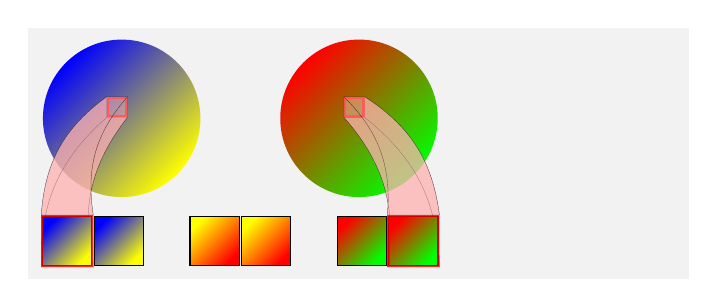
\begin{tikzpicture}[framed, background rectangle/.style={thin, fill=black!5}]
    \begin{pgfonlayer}{bglower}
        \begin{scope}
            \node[anchor=west, blue,  minimum width=2cm, circle] (c1) [left color=blue, right
            color=yellow, shading angle=45] {};%
            \node[green, minimum width=2cm, circle, right=of c1] (c2) [left color=red,  right
            color=green,  shading angle=45] {};%
        \end{scope}
    \end{pgfonlayer}
    \begin{pgfonlayer}{lower}
        \begin{scope}[x=(c1.south west), y=(c1.north east), overlay]
            \node[rectangle, minimum width=0.1cm, minimum height=0.1cm, draw, red, thick] at (0.3, 0.5)
            (r1) {};
            \node[rectangle, minimum width=0.1cm, minimum height=0.1cm, draw, red, thick, shift=($(c2)-(c1)$)] at (0.3, 0.5)
            (r2) {};
        \end{scope}
    \end{pgfonlayer}
    \coordinate (width1) at ($(c2.east)-(c1.west)$);
    \ExtractCoordinate{width1}
    \setlength{\firstscope}{\XCoord}
    % fake scope
    \begin{scope}[opacity=0.0, overlay]
        \node[anchor=west, rectangle, draw, black, minimum width=1cm, minimum height=1cm] (f1) {};
        \node[rectangle, draw, black, minimum width=1cm, minimum height=1cm, right=of f1.west, xshift=0.5mm] (f2) {};
        \node[rectangle, draw, black, minimum width=1cm, minimum height=1cm, right=of f1.west, xshift=2cm] (f3) {};
        \node[rectangle, draw, black, minimum width=1cm, minimum height=1cm, right=of f3.west, xshift=0.5mm] (f4) {};
        \node[rectangle, draw, black, minimum width=1cm, minimum height=1cm, right=of f3.west, xshift=2cm] (f5) {};
        \node[rectangle, draw, black, minimum width=1cm, minimum height=1cm, right=of f5.west, xshift=0.5mm] (f6) {};
    \end{scope}
    \coordinate (width2) at ($(f6.east)-(f1.west)$);
    \ExtractCoordinate{width2}
    \setlength{\secondscope}{\XCoord}
    \pgfmathsetmacro{\ratio}{\firstscope/\secondscope}
    % real scope
    \begin{pgfonlayer}{upper}
        \begin{scope}[scale=\ratio, yshift=-2.5cm]
            \node[anchor=west, rectangle, draw, black, minimum width=1cm, minimum height=1cm,
            transform shape, yellowblue] (t1) {};
            \node[rectangle, draw, black, minimum width=1cm, minimum height=1cm, right=of t1.west,
            xshift=0.5mm, transform shape, yellowblue] (t2) {};
            \node[rectangle, draw, black, minimum width=1cm, minimum height=1cm, right=of t1.west,
            xshift=2cm, transform shape, yellowred] (t3) {};
            \node[rectangle, draw, black, minimum width=1cm, minimum height=1cm, right=of t3.west,
            xshift=0.5mm, transform shape, yellowred] (t4) {};
            \node[rectangle, draw, black, minimum width=1cm, minimum height=1cm, right=of t3.west,
            xshift=2cm, transform shape, greenred] (t5) {};
            \node[rectangle, draw, black, minimum width=1cm, minimum height=1cm, right=of t5.west,
            xshift=0.5mm, transform shape, greenred] (t6) {};
        \end{scope}
    \end{pgfonlayer}
    \begin{pgfonlayer}{upper}
        \begin{scope}[overlay]
            \node[rectangle, inner sep=0mm, red, draw, thick, fit=(t1), opacity=0.8] (r3) {};
            \node[rectangle, inner sep=0mm, red, draw, thick, fit=(t6), opacity=0.8] (r4) {};
        \end{scope}
    \end{pgfonlayer}
    \begin{pgfonlayer}{lower}
        \begin{scope}[opacity=0.5]
            \path[ultra thin, draw, black!100, fill=red!30] (r1.north west) to[bend right=25]
            (r3.north west) to (r3.south west) to[bend left=25]
            (r1.south west) to (r1.north west) -- cycle;
            \path[ultra thin, draw, black!100, fill=red!30] (r1.south east) to (r1.south west)
            to[bend right=25] (r3.south west) to
            (r3.south east) to[bend left=25] (r1.south east) -- cycle;
            \path[ultra thin, draw, black!100, fill=red!30] (r1.south east) to (r1.north east)
            to[bend right=25] (r3.north east) to
            (r3.south east) to[bend left=25] (r1.south east) -- cycle;
            \path[ultra thin, draw, black!100, fill=red!30] (r1.north east) to (r1.north west)
            to[bend right=25] (r3.north west) to
            (r3.north east) to[bend left=25] (r1.north east) -- cycle;

            \path[ultra thin, draw, black!100, fill=red!30] (r2.north west) to[bend right=-25]
            (r4.north west) to (r4.south west) to[bend left=-25]
            (r2.south west) to (r2.north west) -- cycle;
            \path[ultra thin, draw, black!100, fill=red!30] (r2.south east) to (r2.south west)
            to[bend right=-25] (r4.south west) to
            (r4.south east) to[bend left=-25] (r2.south east) -- cycle;
            \path[ultra thin, draw, black!100, fill=red!30] (r2.south east) to (r2.north east)
            to[bend right=-25] (r4.north east) to
            (r4.south east) to[bend left=-25] (r2.south east) -- cycle;
            \path[ultra thin, draw, black!100, fill=red!30] (r2.north east) to (r2.north west)
            to[bend right=-25] (r4.north west) to
            (r4.north east) to[bend left=-25] (r2.north east) -- cycle;
        \end{scope}
    \end{pgfonlayer}
\end{tikzpicture}
\end{document}


